
%(BEGIN_QUESTION)
% Copyright 2009, Tony R. Kuphaldt, released under the Creative Commons Attribution License (v 1.0)
% This means you may do almost anything with this work of mine, so long as you give me proper credit

Read and outline the ``Displacement Interface Level Measurement'' subsection of ``Displacement'' section of the ``Continuous Level Measurement'' chapter in your {\it Lessons In Industrial Instrumentation} textbook.  Note the page numbers where important illustrations, photographs, equations, tables, and other relevant details are found.  Prepare to thoughtfully discuss with your instructor and classmates the concepts and examples explored in this reading.

\vskip 10pt

Make special note of the ``thought experiment'' problem-solving technique applied to the solution of calibration points for liquid-liquid interface level instruments.

\underbar{file i03959}
%(END_QUESTION)





%(BEGIN_ANSWER)


%(END_ANSWER)





%(BEGIN_NOTES)

Just like hydrostatic DP instruments, the only way to measure liquid-liquid interface levels with a displacer instrument is to ensure the total liquid level never drops down into the instrument's measurement range.  This means the displacer cage must {\it always} be completely flooded.

\vskip 10pt

A straight-forward way to calculate LRV and URV range points is to perform a pair of ``thought experiments'' for every instrument: one where the liquid-liquid interface is at the LRV point, and another where the liquid-liquid interface is at the URV point.  In each simulation, calculate the total buoyant force seen by the displacer.  Once the LRV and URV points are determined, any calibration points in between may be determined by interpolation.










\vskip 20pt \vbox{\hrule \hbox{\strut \vrule{} {\bf Suggestions for Socratic discussion} \vrule} \hrule}

\begin{itemize}
\item{} Suppose a cage-style displacer level transmitter is correctly measuring a liquid-liquid interface level, then a technician closes the two block valves and drains the cage of all liquid.  Are there any special procedures for placing the transmitter back into service, or can the technician open the block valves with impunity?
\item{} Can a cageless style of displacer level transmitter be used to measure liquid-liquid interface levels?  Why or why not?
\end{itemize}












\vfil \eject

\noindent
{\bf Summary Quiz:}

Calculate the amount of weight registered by the scale:

$$\includegraphics[width=15.5cm]{i03959x02.eps}$$

\begin{itemize}
\item{} 51.79 lb
\vskip 5pt 
\item{} 45.94 lb
\vskip 5pt 
\item{} 50.92 lb
\vskip 5pt 
\item{} 52.38 lb 
\end{itemize}












%INDEX% Reading assignment: Lessons In Industrial Instrumentation, Continuous Level Measurement (interface level measurement using displacers)

%(END_NOTES)


